
%(BEGIN_QUESTION)

Hydrogenreforming er en prosess der spesielle brennkammer brukes for å lage rent hydrogen fra hydrocarboner. Metan gass (CH$_{4}$) blandes med damp (H$_{2}$O) under høy  temperatur. Da dannes H$_{2}$) og karbonmonodksyd (CO), som i gjen omformes til CO$_{2}$. Denne reaksjonen er endotermisk, som vil si at den krever energi. Denne energien tilføres i et brennkammer. 

$$\includegraphics[width=15.5cm]{i02504x01.eps}$$

Mengden hydrokarboner som tilføres prosessen påvirker i høy grad temperaturen inne i forbrenningskammeret, noe som gjør det utfordrende å holde temperaturen på settpunktet. Skisser en løsning på dette temperaturstabilitetsproblemet ved å bruke forkover koblet regulering. 
%The rate of hydrocarbon feed greatly ``loads'' the control of temperature inside the reaction furnace, making it more challenging to maintain setpoint temperature as the feed rate varies.  Design a solution for this temperature-stability problem using a {\it feedforward} control strategy, explaining the reasoning behind your solution.



b) En prosess gir følgende graf ved et sprang i pådraget

$$\includegraphics[width=15.5cm]{i01662x01.eps}$$

Hvilken type prosess er dette?


c) En prosess gir følgende graf ved et sprang i pådraget

$$\includegraphics[width=15.5cm]{i01663x01.eps}$$

Hvilken type prosess er dette?

d) Regn ut følgende basert på at transmitteren er kalibrert for et måleområde fra 50mbar til 400mbar. Transmitteren har et utgangssignal på 4-20mA \\
Vis alle utregninger. \\
$$\includegraphics[width=15.5cm]{i04815x02.eps}$$



\begin{itemize}
\item{} $I$ = \underbar{\hskip 50pt} mA
\vskip 10pt
\item{} $U_{C}$ = \underbar{\hskip 50pt} V 
\vskip 10pt
\item{} $U_{BC}$ = \underbar{\hskip 50pt} V 
\vskip 10pt
\item{} $U_{B}$ = \underbar{\hskip 50pt} V 
\end{itemize}

\filbreak

%\vfil
%\underbar{file i00000}
%\eject
%(END_QUESTION)





%(BEGIN_ANSWER)


%(END_ANSWER)





%(BEGIN_NOTES)


%INDEX% Alarm, ???: (word or phrase here)
%INDEX% Basics, transmitter: input and output ranges
%INDEX% Basics, ???: (word or phrase here)
%INDEX% Career, ???: (word or phrase here)
%INDEX% Calibration, table: (word or phrase here)
%INDEX% Calibration, ???: (word or phrase here)
%INDEX% Certification exam: (word or phrase here)
%INDEX% Chemistry, ???: (word or phrase here)
%INDEX% Control, proportional: (word or phrase here)
%INDEX% Control, derivative: (word or phrase here)
%INDEX% Control, integral: (word or phrase here)
%INDEX% Control, process characteristics: (word or phrase here)
%INDEX% Control, proportional + derivative: (word or phrase here)
%INDEX% Control, proportional + integral: (word or phrase here)
%INDEX% Control, proportional + integral + derivative: (word or phrase here)
%INDEX% Control, PID tuning: (word or phrase here)
%INDEX% Control, strategies: (word or phrase here)
%INDEX% Control, ???: (word or phrase here)
%INDEX% Course organization, ???: (word or phrase here)
%INDEX% Data Acquisition, ???: (word or phrase here)
%INDEX% DCS, ???: (word or phrase here)
%INDEX% Documentation, P&ID: (word or phrase here)
%INDEX% Documentation, loop diagram: (word or phrase here)
%INDEX% Documentation, functional: (word or phrase here)
%INDEX% Documentation, ???: (word or phrase here)
%INDEX% Electronics review: (word or phrase here)
%INDEX% Fieldbus, ???: (word or phrase here)
%INDEX% Final Control Elements, valve: (word or phrase here)
%INDEX% Final Control Elements, motor: (word or phrase here)
%INDEX% Final Control Elements, pump: (word or phrase here)
%INDEX% Good practices, wiring: ???
%INDEX% Good practices, ???: ???
%INDEX% Lab exercise, ???
%INDEX% Mathematics, calculus: (word or phrase here)
%INDEX% Mathematics, probability: (word or phrase here)
%INDEX% Measurement, pressure: (word or phrase here)
%INDEX% Measurement, level: (word or phrase here)
%INDEX% Measurement, temperature: (word or phrase here)
%INDEX% Measurement, flow: (word or phrase here)
%INDEX% Measurement, analytical: (word or phrase here)
%INDEX% Measurement, ???: (word or phrase here)
%INDEX% Mechanics, pneumatic instrument: (word or phrase here)
%INDEX% Mechanics, ???: (word or phrase here)
%INDEX% Networking, ???: (word or phrase here)
%INDEX% Physics, units and conversions: (word or phrase here)
%INDEX% Physics, energy, work, power: (word or phrase here)
%INDEX% Physics, static fluids: (word or phrase here)
%INDEX% Physics, temperature: (word or phrase here)
%INDEX% Physics, dynamic fluids: (word or phrase here)
%INDEX% Physics, ???: (word or phrase here)
%INDEX% PLC, ???: (word or phrase here)
%INDEX% Relay, ???: (word or phrase here)
%INDEX% Safety, ???: (word or phrase here)
%INDEX% Switch, pressure: (word or phrase here)
%INDEX% Switch, level: (word or phrase here)
%INDEX% Switch, temperature: (word or phrase here)
%INDEX% Switch, flow: (word or phrase here)
%INDEX% Switch, ???: (word or phrase here)
%INDEX% Troubleshooting circuit, ???

%(END_NOTES)


